\edef\indentacao{\the\parindent}

\noindent
\begin{minipage}[t]{0.55\textwidth}\setlength{\parindent}{\indentacao}

    Para os casos em que é necessário apresentar dados com mais de uma váriavel dependente de um mesmo dado \texttt{X}, existe a opção de gráficos múltiplos. Eles servem para comparar as relações do tipo $y_1 = f(x)$ e $y_2 = g(x)$, quando $x$, $y_1$ e $y_2$ são medidos em conjunto.

    Em experimentos com circuitos, esse tipo de dado aparece, por exemplo, na medição de tensão em nós diferentes para a comparação de seus comportamentos no tempo. É o caso do circuito da figura \ref{fig:multiv:circuito}, cujos dados foram colocados como na figura \ref{fig:multiv:dados}.

    \begin{figure}[H]
        \centering
        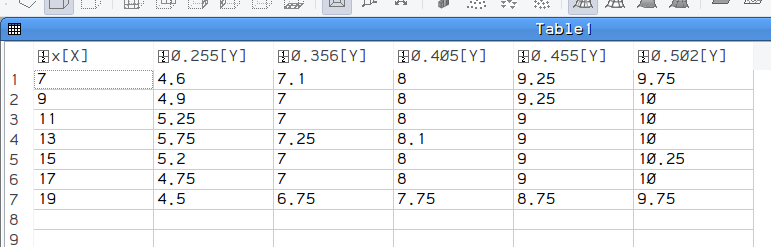
\includegraphics[width=0.8\textwidth]{multiv/1dados.png}

        \caption{Dados gerados com simulador}
        \label{fig:multiv:dados}
    \end{figure}

\end{minipage}\vspace{0.05\textwidth}%
\begin{minipage}[t]{0.4\textwidth}
    \begin{figure}[H]
        \centering
        \begin{circuitikz}[scale=1.2]

    \draw (2, 0)
    to [short] ++(-2,0)
    to [vsourcesin, l=$E$] ++(0,4)
    to [short] ++(2,0)
    to [resistor, l_=$R$] ++(0,-2)
    to [capacitor, l_=$C$] ++(0,-2)
    node[ground] {};

    \draw [->, thick] (3,4) to node[above] {$V_1$} (2.1,4);

    \draw [->, thick] (3,2) to node[above] {$V_2$} (2.1,2);

\end{circuitikz}


        \caption{Circuito de defasagem de tensão por um capacitor}
        \label{fig:multiv:circuito}
    \end{figure}
\end{minipage}


\subsection{Gráficos de Eixos Separados}

    Uma opção para mostrar os dois canais ao mesmo tempo é colocar cada um em seu próprio gŕafico com seus próprios eixos. No \software, isso é feito como na figura \ref{fig:multiv:paneis:tutorial}, mas pode ser feito em duas imagens separadas também. O problema com essa abordagem é que as escalas diferentes não mostram muito bem as proporções entre os canais de entrada e saída.

    \begin{figure}[H]
        \centering
        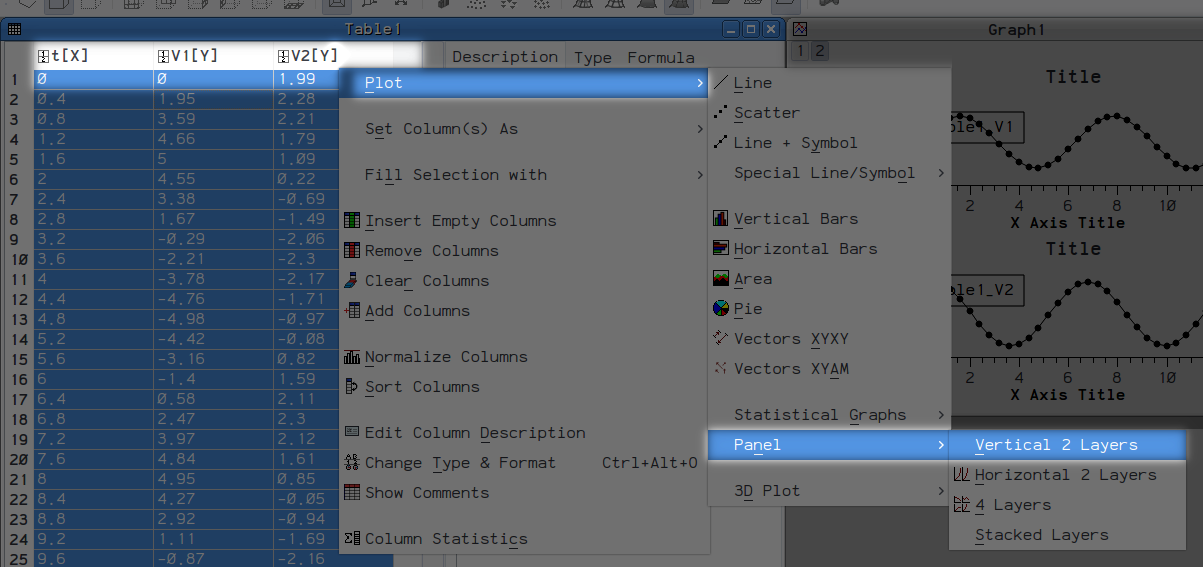
\includegraphics[width=0.6\textwidth]{multiv/2paneis.png}

        \caption{Criando os gráficos separados}
        \label{fig:multiv:paneis:tutorial}
    \end{figure}

    \begin{figure}[H]
        \centering
        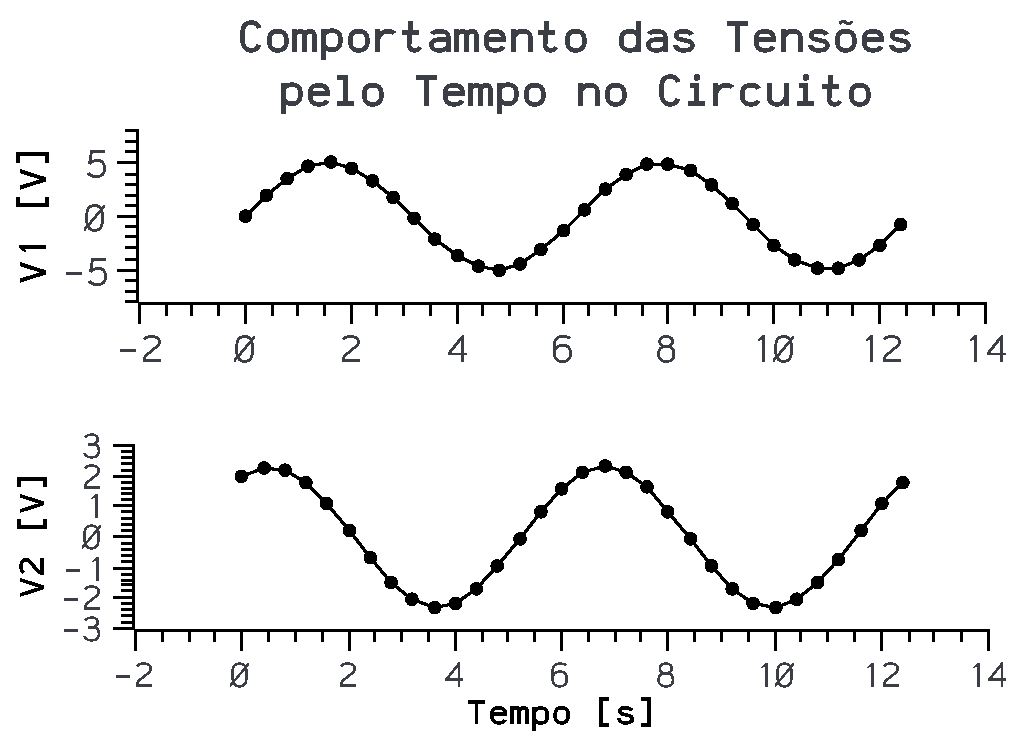
\includegraphics[width=0.6\textwidth]{multiv/3paneis.pdf}

        \caption{Gráficos das tensões de entrada e saída do circuito}
        \label{fig:multiv:paneis}
    \end{figure}


\subsection{Gráficos de Eixos em Conjunto} \label{sec:multiv:juntos}

    \begin{figure}[htbp]
        \centering
        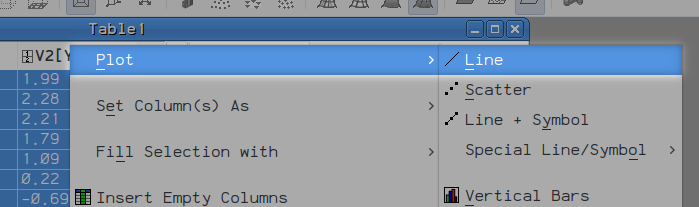
\includegraphics[width=0.6\textwidth]{multiv/4dois.png}

        \caption{Criando o gráfico com as duas curvas}
        \label{fig:multiv:juntos:tutorial}
    \end{figure}

    Esse método é melhor para visualizar a diferença de escala entre os dados, mas, se algum dos dados tem uma escala muito diferente, o gráfico pode acabar perdendo na percepção dos dados. Um dos maiores limites para esse método, no entanto, é que as variáveis dependentes precisam ter a mesma motivação física e, por causa disso, a mesma gradeza, caso contrário, o eixo compartilhado entre elas perde completamente o sentido.

    \begin{figure}[htbp]
        \centering
        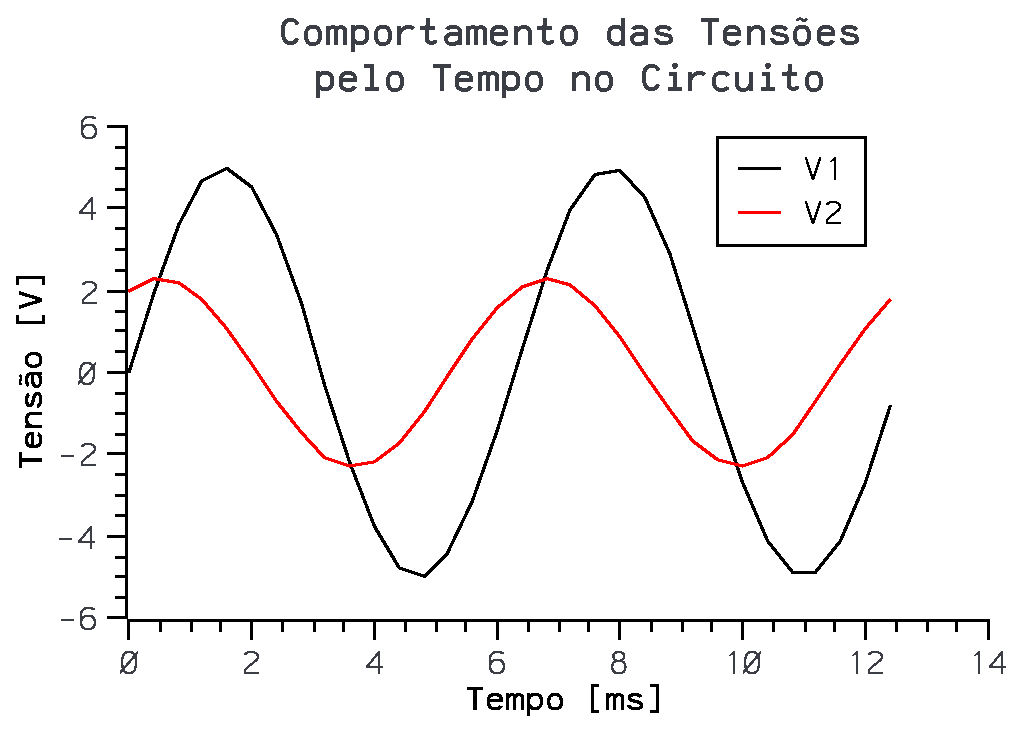
\includegraphics[width=0.6\textwidth]{multiv/5dois.pdf}

        \caption{Gráfico em conjunto das tensões $V_1$ e $V_2$ do circuito}
        \label{fig:multiv:juntos}
    \end{figure}


\subsection{Gráficos com Apenas a Abscissa Comum}

    \begin{figure}[htbp]
        \centering
        \begin{subfigure}{0.35\textwidth}
            \centering
            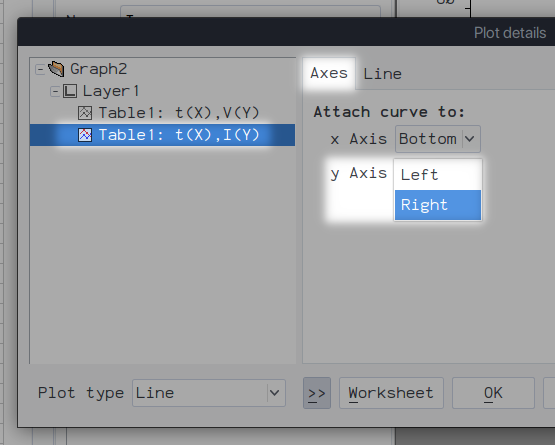
\includegraphics[width=\textwidth]{multiv/6duplo.png}

            \caption{Alterando o eixo da corrente como um eixo separado}
            \label{fig:multiv:duplo:eixo}
        \end{subfigure}
        ~
        \begin{subfigure}{0.6\textwidth}
            \centering
            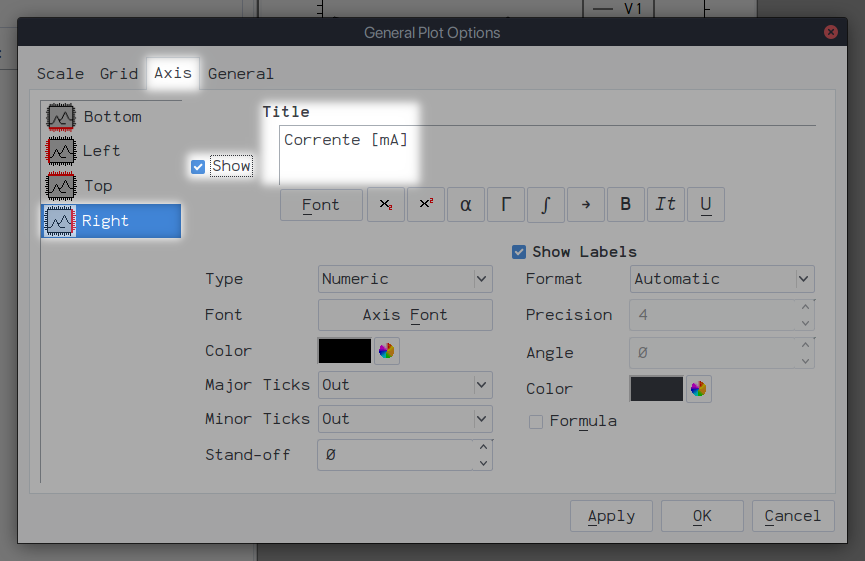
\includegraphics[width=\textwidth]{multiv/7eixo.png}

            \caption{Mostrando o novo eixo da corrente}
            \label{fig:multiv:duplo:eixado}
        \end{subfigure}
        \caption{Criando o gráfico com três eixos}
        \label{fig:multiv:duplo:tutorial}
    \end{figure}

    Imagine agora o caso em que queremos mostrar a defasagem entre a corrente a tensão no capacitor da figura \ref{fig:multiv:circuito}. A única grandeza comum agora é o tempo, então vamos precisar de gráficos de três eixos. No \software, isso é feito como na seção \nameref{sec:multiv:juntos}, com as alterações mostradas nas imagems \ref{fig:multiv:duplo:eixo} e \ref{fig:multiv:duplo:eixado}. Normalmente, é melhor alterar as cores para melhor representar cada dado.

    \begin{figure}[htbp]
        \centering
        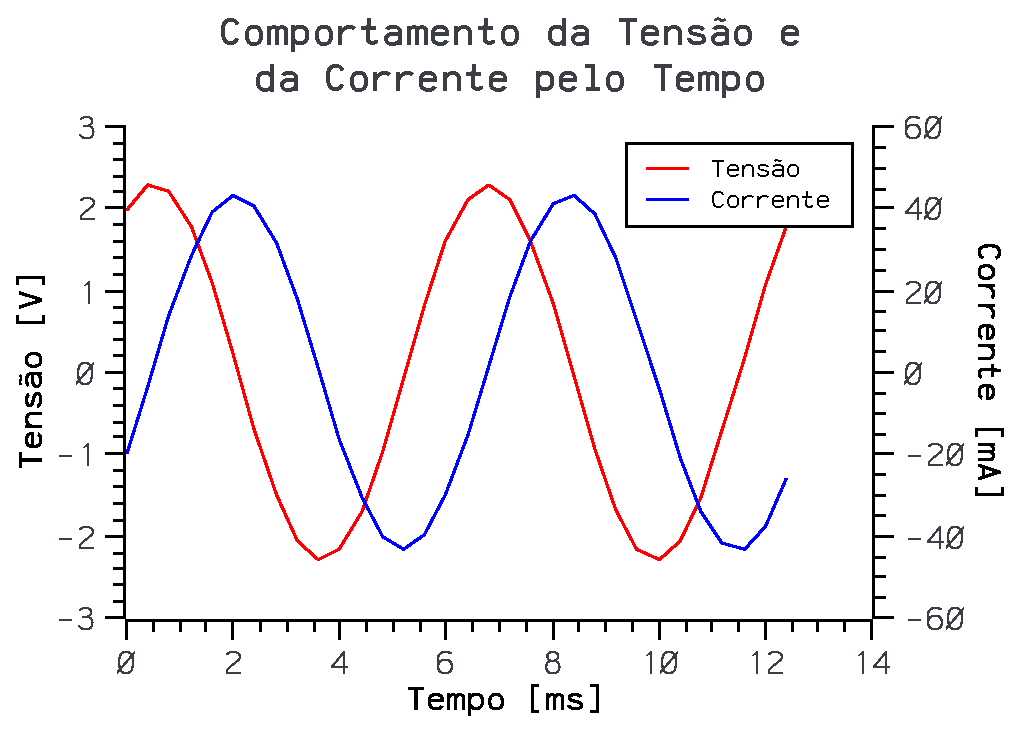
\includegraphics[width=0.6\textwidth]{multiv/8duplo.pdf}

        \caption{Gráfico de corrente e tensão por tempo no capacitor (circuito \ref{fig:multiv:circuito})}
        \label{fig:multiv:duplo}
    \end{figure}

    \begin{nota}
        As vezes, os gráficos com múltiplas curvas podem ficar sobrecarregados de informação. Quando isso acontece, o melhor é separar os dados em gráficos distintos pra manter a legibilidade. Gráficos de três eixos pdem ficar complicados com facilidade.
    \end{nota}
